\documentclass{chi-ext}
% Please be sure that you have the dependencies (i.e., additional LaTeX packages) to compile this example.
% See http://personales.upv.es/luileito/chiext/

%% EXAMPLE BEGIN -- HOW TO OVERRIDE THE DEFAULT COPYRIGHT STRIP -- (July 22, 2013 - Paul Baumann)
% \copyrightinfo{Permission to make digital or hard copies of all or part of this work for personal or classroom use is granted without fee provided that copies are not made or distributed for profit or commercial advantage and that copies bear this notice and the full citation on the first page. Copyrights for components of this work owned by others than ACM must be honored. Abstracting with credit is permitted. To copy otherwise, or republish, to post on servers or to redistribute to lists, requires prior specific permission and/or a fee. Request permissions from permissions@acm.org. \\
% {\emph{CHI'14}}, April 26--May 1, 2014, Toronto, Canada. \\
% Copyright \copyright~2014 ACM ISBN/14/04...\$15.00. \\
% DOI string from ACM form confirmation}
%% EXAMPLE END -- HOW TO OVERRIDE THE DEFAULT COPYRIGHT STRIP -- (July 22, 2013 - Paul Baumann)

\title{Gesture Typing on Virtual Tabletop: Effect of Input on Performance}

\numberofauthors{4}
% Notice how author names are alternately typesetted to appear ordered in 2-column format;
% i.e., the first 4 autors on the first column and the other 4 auhors on the second column.
% Actually, it's up to you to strictly adhere to this author notation.
\author{
  \alignauthor{
    \textbf{First Author}\\
    \affaddr{AuthorCo, Inc.}\\
    \affaddr{123 Author Ave.}\\
    \affaddr{Authortown, PA 54321 USA}\\
    \email{author1@anotherco.com}
  }\alignauthor{
    \textbf{Fourth Author}\\
    \affaddr{AuthorCo, Inc.}\\
    \affaddr{123 Author Ave.}\\
    \affaddr{Authortown, PA 54321 USA}\\
    \email{author5@anotherco.com}
  }
  \vfil
  \alignauthor{
    \textbf{Second Author}\\
    \affaddr{AuthorCo, Inc.}\\
    \affaddr{123 Author Ave.}\\
    \affaddr{Authortown, PA 54321 USA}\\
    \email{author2@anotherco.com}
  }\alignauthor{
    \textbf{Fifth Author}\\
    \affaddr{AuthorCo, Inc.}\\
    \affaddr{123 Author Ave.}\\
    \affaddr{Authortown, PA 54321 USA}\\
    \email{author6@anotherco.com}
  }
\vfil
}

% Paper metadata (use plain text, for PDF inclusion and later re-using, if desired)
\def\plaintitle{Gesture Typing on Virtual Tabletop: Effect of Input on Performance}
\def\plainauthor{Name}
\def\plainkeywords{Gesture Input, Gesture Keyboard, Mobile, Continuous Interaction, Tabletop, Text Input}
\def\plaingeneralterms{Documentation, Standardization}

\hypersetup{
  % Your metadata go here
  pdftitle={\plaintitle},
  pdfauthor={\plainauthor},
  pdfkeywords={\plainkeywords},
  pdfsubject={\plaingeneralterms},
  % Quick access to color overriding:
  %citecolor=black,
  %linkcolor=black,
  %menucolor=black,
  %urlcolor=black,
}

\usepackage{graphicx}   % for EPS use the graphics package instead
\usepackage{balance}    % useful for balancing the last columns
\usepackage{bibspacing} % save vertical space in references

\usepackage{subfigure}

% own command
\newcommand{\reffigure}[1]{Figure~\ref{#1}}
\newcommand{\reftable}[1]{Table~\ref{#1}}
\newcommand{\smit}[1]{{\small\textit{{#1}}}}
\newcommand{\cdt}[1]{{\small\uppercase{{#1}}}}
\newcommand{\wpm}{\cdt{wpm} }


\begin{document}

\maketitle

\begin{abstract}
Gesture typing performed through tabletop interaction presents potential for severely/physically impaired users. In this work, we use virtual touch surfaces to bring gesture typing interaction to a tabletop scenario. We first report on the prototype developed and follow with a user study that compares our interaction technique to a control tablet scenario, and explore the influence of input size and aspect ratio on the text input performance. We show that novice user performs at half the rate with our system as compared to control, and that a size of A5/A4 present the best compromise between precision and user preference.
\end{abstract}

\keywords{\plainkeywords}
\textcolor{red}{Optional section to be included in your final version.}

\category{H.5.m}{Information interfaces and presentation (e.g., HCI)}{Miscellaneous}.
%See \cite{ACMCCS}
See: \url{http://www.acm.org/about/class/1998/}
for help using the ACM Classification system.
\textcolor{red}{Optional section to be included in your final version, but strongly encouraged.}

\begin{figure}
    \centering
    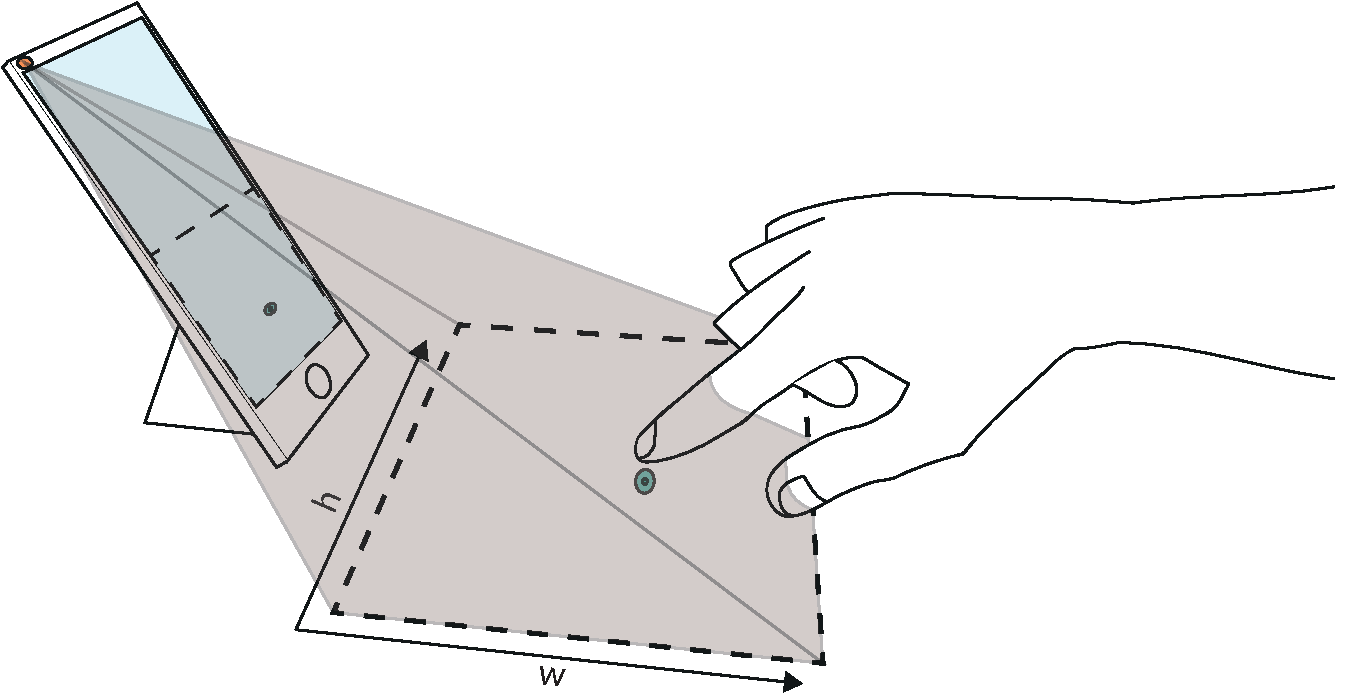
\includegraphics[width=\linewidth]{figures/banner.pdf}
    \caption{Potential interaction setup. A mobile device whose optical sensor creates an on-demand touch surface offers two degrees of freedom in the choice of surface geometry.}~\label{fig:banner}
\end{figure}
\marginpar{
\begin{figure}
  \begin{center}
  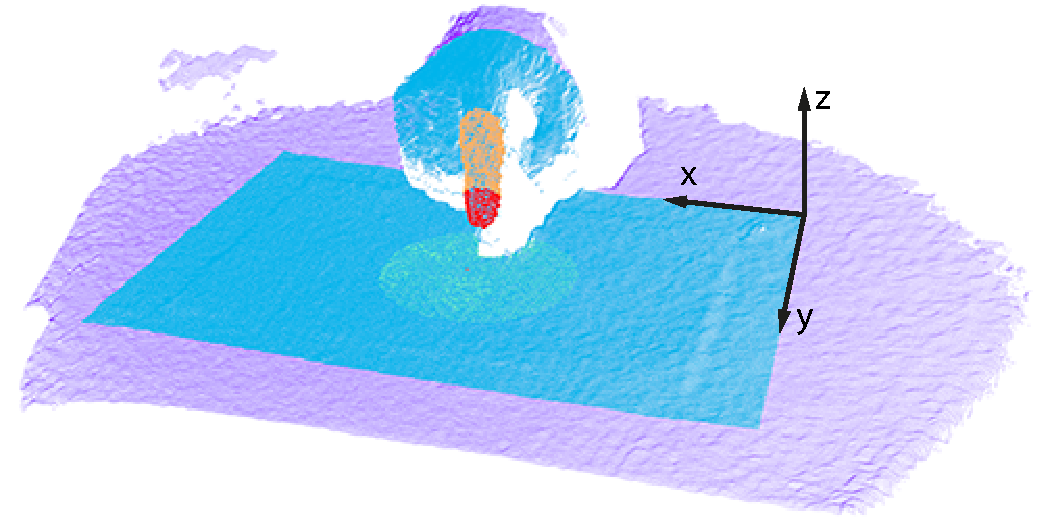
\includegraphics[width=\marginparwidth]{figures/pointcloud.pdf}
  \caption{Real segmented sensor image from our prototype with in blue the points within the interactive surface, in cyan the ROI plane, in yellow the detected fingers and in red the user pointer.}
  \label{fig:marginparsample}
  \end{center}
\end{figure}
}
% =============================================================================
\section{Introduction}
% =============================================================================

The commoditization of depth camera creates opportunity for novel interaction scenarios. From its inception with Omnitouch~\cite{Harrison2011} to more recent work, such as Xiao et al. ~\cite{Xiao2016}, using vision-based system for tabletop interaction affords economy and flexible designs. Virtual surfaces are indeed parametrisable, tackle the palm rejection problem and among others allow for dirty hand/sterile scenarios.

This can be interesting for patients with severe physical disabilities. The flexibility of such a system allow for rapid deployment but also let the designer finding the best parameters for the interaction in terms of size and touch point. Moreover, tabletop interaction is nice to the body since it allows to the forearm during the interaction.

Given that text-input remains a very important activity on mobile devices~\cite{McGregor2014}, we set out to explore the feasibility of gesture typing~\cite{Kristensson2004} on the prototype as it suits well our interaction paradigm.

This work aims at making the following two specific contributions:
\begin{itemize}
\item we describe supervised learning solution to the fingertip touch classification problem.
\item we analyse the influence of input space in terms of size and aspect ratio on the gesture typing performance.
\end{itemize}

% =============================================================================
\section{System overview}
% =============================================================================

Before implementing a prototype, we gathered some feedback from a Wizard of Oz testing where 4 participants with high spinal cord injury performed gesture typing like shapes on a tabletop. We gained the insights that this user group is capable of performing the said trajectories, up to A4/A3 and that

The field of hand pose estimation is rapidly moving, and at the time of the study we did not find a software package that would fill all the requirements. We chose to perform simple hand tracking with Kalman filtering of the closest point to the camera, and did spend some time on the touch classification - which (is rarely tackled/has proven problematic) in the litterature~\cite{Xiao2016}.

This problem is usually solved by manually setting threshold from observation from the data. This is however very well suited for a supervised learning scheme. With that in mind, we recorded 12 minutes of film, equally balanced with touching and non-touching frames, as well as different fingers (pinky, middle and index) and different pose angle. We trained a simple MLP classifier.

\begin{figure}
    \centering
    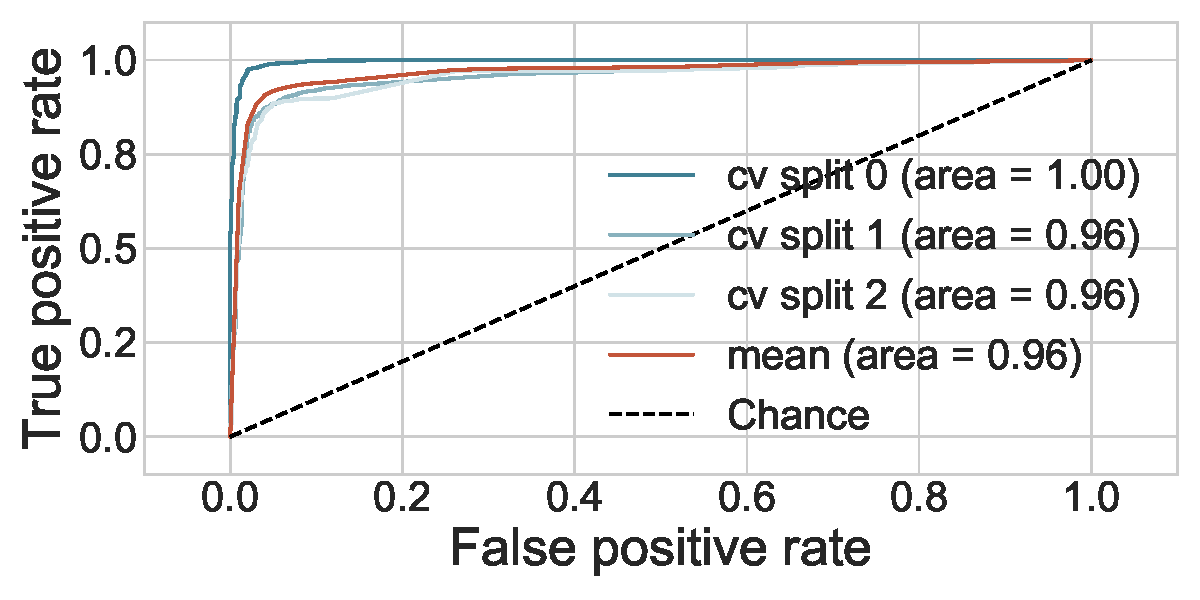
\includegraphics[width=\linewidth]{figures/roc_auc.pdf}
    \caption{Performance of the fingertip touch classification based on a classic supervised machine learning algorithm.}~\label{fig:banner}
\end{figure}

From the recording camera, and after processing on a stationnary computer (in soft realtime), the detected touch events as sent to a mobile device which runs a custom application and reacts as if the user was touching the screen. An additional audiovisual feedback is presented to display hover position and touch down events.

% =============================================================================
\section{User study}
% =============================================================================
We designed a user study with two goals in mind, evaluating the usiability of the system as compared to an interaction on a mobile device, and finding out the influence of the size and aspect ratio of the input surface onto the text input rate. The design is detailed in table.

We gathered 12 participants, all right handed, only one had previous experience with gesture typing.
We  balanced the LEVEL condition. The task was to write in succession 20 words taken at random from the most common english words with length between 2 and 5 letters\footnote{Word sample used for the experiment: \{\cdt{asset}, \cdt{badly}, \cdt{chew}, \cdt{deck}, \cdt{dog}, \cdt{end}, \cdt{fix}, \cdt{gate}, \cdt{herb}, \cdt{hide}, \cdt{hot}, \cdt{iron}, \cdt{lab}, \cdt{lay}, \cdt{order}, \cdt{safe}, \cdt{seek}, \cdt{seem}, \cdt{want}, \cdt{wrong}\}}. The design of the task allow the user to familiarise with gesture typing and emulates a proficient bahavior. We also asked the user to fill in a NASA Task Load Index.

\begin{table}
  \centering
  \begin{tabular}{l l | r r r r r}
    \smit{LEVEL} & \smit{DEVICE} & \smit{width} & \smit{height} & \smit{area}& \smit{ratio} & \smit{$CD_{gain}$} \\
    % \midrule
    \hline
    \cdt{OP1} & \cdt{optical} & 9.4 & 4.7 & 44.2 & 2 & 1 \\
    \cdt{OP2} & \cdt{optical} & 18.8 & 9.4 & 176.7 & 2 & 1/2 \\
    \cdt{OL2} & \cdt{optical} & 25.6 & 6.9 & 176.6 & 3.7 & 1/1.7 \\
    \cdt{OP4} & \cdt{optical} & 37.7 & 18.9 & 712.5 & 2 & 1/4 \\
    % \midrule
    \hline
    \cdt{tp1} & \cdt{tablet} & 9.4 & 4.7 & 44.2 & 2 & 1 \\
    % \bottomrule
  \end{tabular}
  \caption{Dimensions in centimeters, area in squared centimeter, ratio and control/display gain for all 5 combinations used in the experiment.}~\label{tab:cdt}
\end{table}

% =============================================================================
\section{Preliminary result}
% =============================================================================
We measure the dependent variable time to completion and ...
The dependent variables are the success rate, the time taken per trial and the trace data when available. This allowed us to compute the dependent measure error rate defined as the per- centage of unsucessful attempts as well as the text entry rate measured in Words Per Minute (WPM), as in [3], according to the formula: $WPM = |T|/s \times 60/5$ where $|T|$ is the length of the transcribed string, s is time in seconds.

We found that LAY presented some very unusual behavior. Entry rates had an error rate at $89.5\%$ while the WORD mean is $20.1\%$ and no other word had an error rate higher than $30\%$. The reason is that the recogniser promotes words of higher prior probability in the language model, in this case “Larry”, “last” or “Katy” - highlight the limitations of pure gesture typing interaction.

A statistical analysis showed a significant main effect of DEVICE (F1,11 = 37.77, p < 0.0001) on error rate with mean value for TP1 and OP1 equal to respectively 6.2\% and 26.1\%, see Figure 4.a. A statistical analysis also showed a significant main effect of SIZE (F2,22 = 10.99, p < 0.001) on the error rate. Finally, an ANOVA on TP1, OP2, OP4 and OL2 did not show a significant main effect (p = 0.11) even though OPTICAL is in average higher than TABLET. In other words, among all levels of the experiment, only OP1 shows a significant higher error rate.

A statistical analysis showed a significant main effect of DEVICE (F1,11 = 90.15, p < 0.0001) on input rate with mean values for TP1 and OP1 equal to respectively 29.2 WPM and 13.7 WPM. We also looked at pair-wise comparison2 for OP-TICAL and could not find a statistical difference in the mean input rate. The input rate achieved by the participants in TP1 is in-line with what can be expected from novice users after the time of the experiments~\cite{Kristensson2004}. The averaged 54\% lower input rate in OPTICAL should be compared with other simi- lar results, as~\cite{Markussen2014} with 57\% after 10 sessions, that compare direct and indirect input modality for mid-air gesture typing.

The participants were capable of moving their hand with great variability when it comes to speed.

The Nasa TLX reported high stress on big surfaces, and high stress on the very small surface. As a results, the optimal size is in the middle.

\begin{figure}
\centering     %%% not \center
\subfigure[]{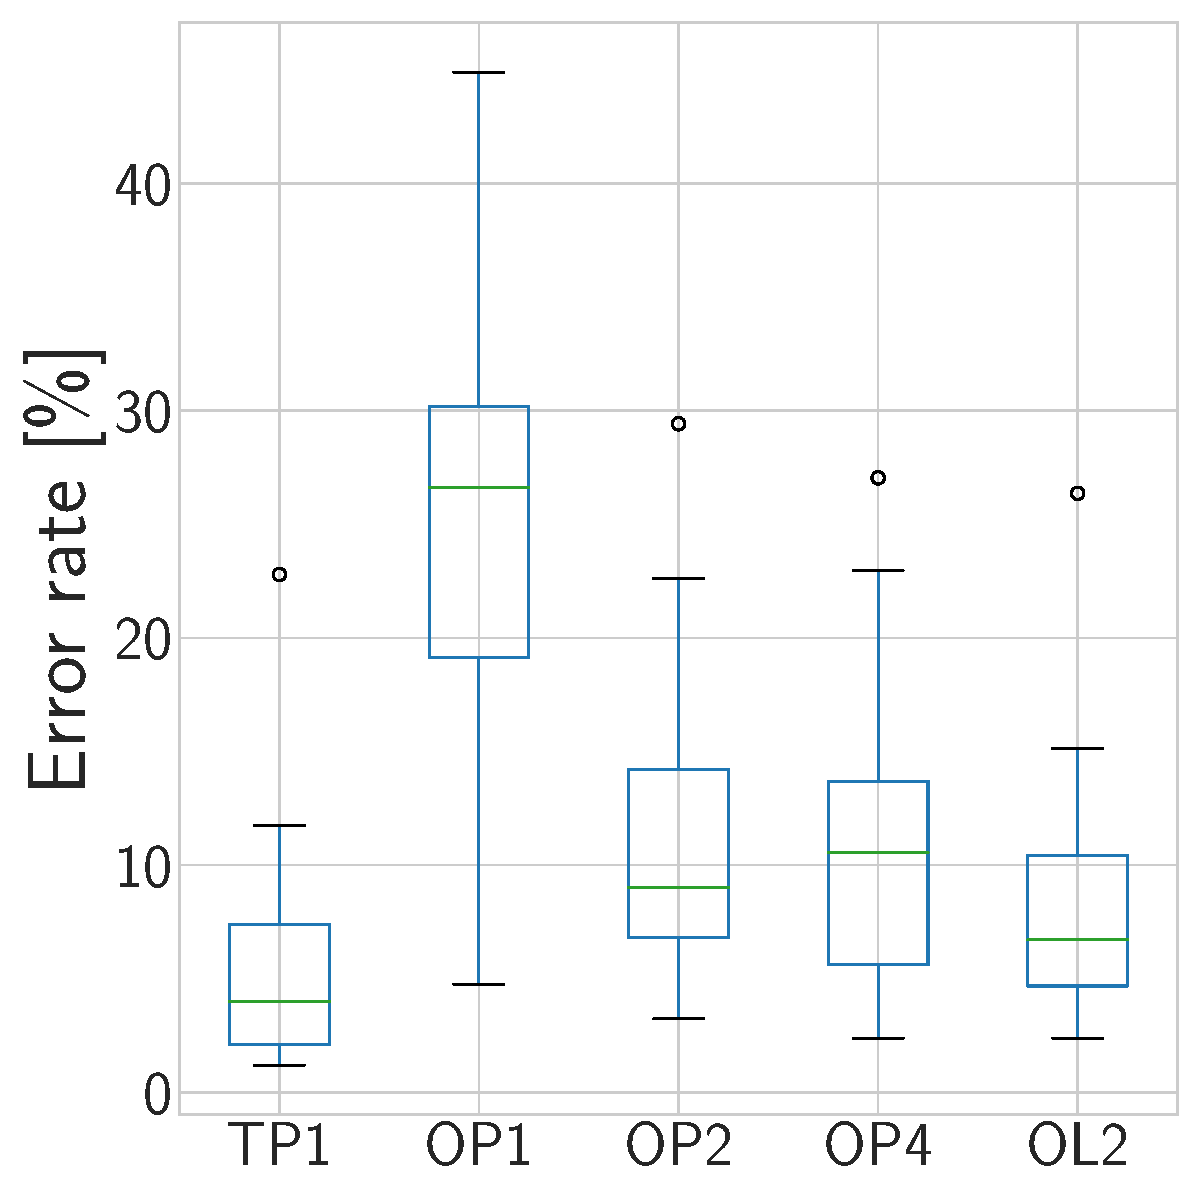
\includegraphics[width=0.49\linewidth]{figures/err_DEVICE_SHAPE.pdf}}
\subfigure[]{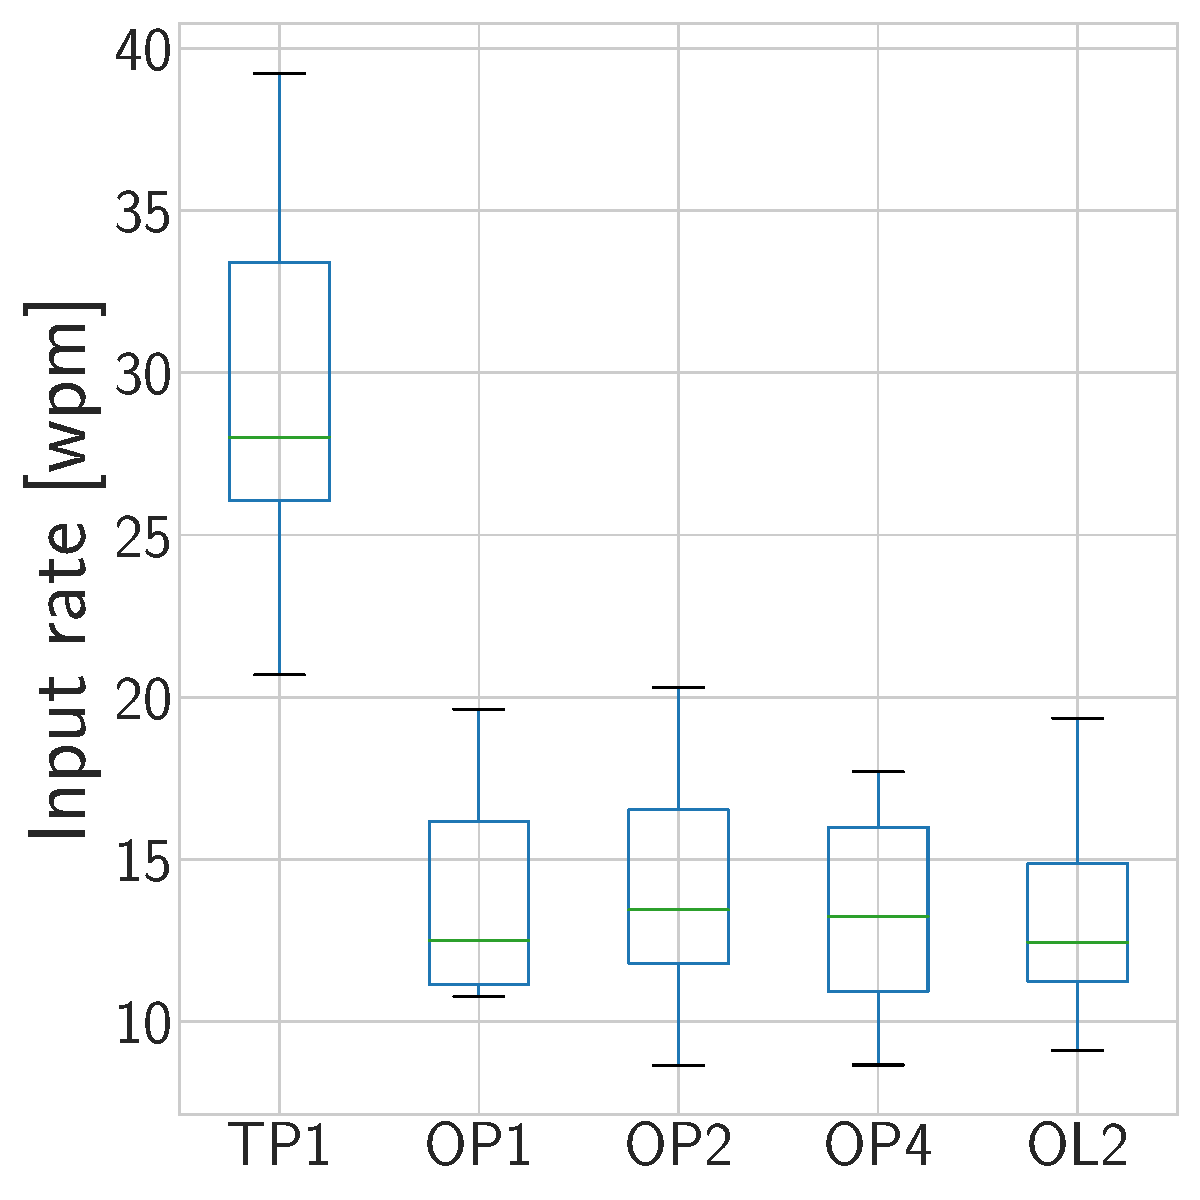
\includegraphics[width=0.49\linewidth]{figures/wpm_DEVICE_SHAPE.pdf}}
\caption{Effect of levels on error rate (a) and input rate (b).}~\label{fig:effect_shape}
\end{figure}

% =============================================================================
\section{Conclusion and Future work}
% =============================================================================
The user study showed that the users hit the accuracy ceiling when using a small surface. It also showed that the task behave according to Fitts law.

The user study These encouraging results open the way to testing the system with patients with spinal cord injury. More so, due to recent advance in hand pose recognition, the reality of interacting via touch through vision based system should be investigated further.

\section{Acknowledgements}
We would like to thank the EU Moregrasp project for funding the research, as well as the patients in the spinal unit in Heidelberg for providing early feedback about the interaction technique.

\balance
\bibliographystyle{acm-sigchi}
\bibliography{collection}

\end{document}